\newcommand{\tituloProblema}[2]{\textbf{\\#1. #2\\}}
\xchapter{Problemas}{}
\acresetall
\label{cap-problemas-textos}
\section{Coleção de músicas}
\tituloProblema{1}{Problema}
Um certo colecionador de arte dispõe de partituras e gravações de
músicas, as quais ele precisa catalogar e processar mediante computador.
O colecionador em questão é muito exigente com o tratamento do seu material e
garante que para cada música na sua coleção, a partitura corresponde exatamente com
a gravação correspondente.

Algumas das partituras que o colecionador possui são para apenas um
instrumento.
Outras são para vários instrumentos.
Cada partitura para um instrumento pode ser vista como uma sequência de
símbolos musicais.
No caso das partituras para vários instrumentos, elas podem ser vistas
como sequências, mas de símbolos compostos: cada elemento da sequência é formado por um número finito
de símbolos musicais.
Cada música pode ter um número arbitrário de símbolos.

Veja a seguir exemplos de partituras.

Um instrumento:\\
\begin{abc}[name=um]
X:1
M:2/4
K:G
[L:1/4] G/A/ | B d | d B | c c |
\end{abc}

Note que cada nota pode ser vista de forma independente como um símbolo (escrito em um pentagrama). No exemplo a seguir, correspondente a uma partitura para três instrumentos, cada um deles possui uma representação similar à vista acima: Cada instrumento possui o seu próprio pentagrama e em cada um deles, os símbolos são superpostos em cada tempo.

Três instrumentos:\\
\begin{abc}[name=tres]
X: 1
M: 3/4
L: 1/4
V:1 name="Flauta" clef=treble
V:2 name="Baixo" clef=treble
V:3 name="Piano" clef=treble
K:Gm
%
[V:1] |: b d' b/g/ | ^f d a
[V:2] |: G B G | d ^f d 
[V:3] |: G/A/ b  B | d A c
\end{abc}

No caso das partituras para vários instrumentos, elas
também podem ser vistas como sequências, mas de símbolos
compostos: cada elemento da sequência é formado
por um número finito de símbolos musicais, sendo um
em cada instrumento.

Apesar de bastante exigente, este colecionador não entende muito bem sobre linguagens,
mas ele gostaria de ter um sistema automatizado que pudesse criar novas composições
a partir das que já possui.

O colecionador ficou sabendo que os alunos desta turma de Introdução as Linguagens Formais
e Teoria da Computação da UFBA estão estudando sobre linguagens formais, então decidiu pedir
ajuda para que eles idealizassem o sistema.

Ele disponibilizou toda a coleção e listou algumas restrições que o sistema
deve atender para que ele fique satisfeito.

\begin{enumerate}
\item O colecionador quer que ao menos duas músicas sejam utilizadas como base para gerar uma nova música,
onde apenas símbolos existentes nas músicas utilizadas como base podem ser utilizadas para uma nova composição;
\item O colecionador gostaria que o sistema fosse capaz de criar músicas para uma quantidade variada de instrumentos;
\item Em ao menos $10\%$ e no máximo $20\%$ das superposições dos símbolos, isto é, quando a nova composição for para mais de um instrumento,
o colecionador gostaria de ouvir a mesma nota em todos os instrumentos da nova composição;
\item O colecionador quer que pequenos trechos das músicas utilizadas como base estejam
presentes nas novas composições;
\item O colecionador quer ter certeza que as novas composições contemplam o máximo
de operações existentes em linguagens formais estudadas pelos alunos, então pediu para
que eles assim fizessem, além de incluir detalhadamente ao menos um exemplo de cada operação
no relatório.
\end{enumerate}

\tituloProblema{2}{Produto}
Uma nova coleção de músicas com no mínimo 10 composições geradas conforme as exigências do colecionador
para demonstrar que é capaz de desenvolver o sistema idealizado, bem como, um relatório no modelo de
artigos da SBC que descreva com o máximo de detalhes a idealização de funcionamento do sistema, onde deverá
constar quais as operações executadas pelo sistema para criação das músicas e incluir ao menos
um exemplo de cada uma das operações sob linguagens formais utilizadas pelo sistema idealizado.

\tituloProblema{3}{Cronograma}
4 sessões tutoriais e 1 aula expositiva.

\tituloProblema{4}{Recursos para aprendizagem}
RAMOS, M. V. M.; JOSÉ NETO, J.; VEGA, I. S. \textbf{Linguagens Formais: Teoria, Modelagem e Implementação}. Editora Bookman, 2009.\\

\noindent
MENEZES, Paulo Blauth. \textbf{Linguagens formais e autômatos}. 6. ed. Bookman, 2011.\\

\noindent
https://hudlac.wordpress.com/notacao-musical-abc\\

\noindent
http://abcnotation.com

\tituloProblema{$*$}{Referências}
Este problema é baseado nas notas de aula do professor Martin Musicante\footnote{\scriptsize{https://sigaa.ufrn.br/sigaa/public/docente/portal.jsf?siape=1221251}} do DIMAP - UFRN.

\newpage
\section{A máquina de vender refrigerantes}
\tituloProblema{1}{Problema}
A empresa \textit{Refrigerantes e Salgados S.A.} resolveu desenvolver novas soluções
para as suas máquinas de vender refrigerantes e salgados
baseadas em autômatos finitos.

A ideia surgiu quando um dos representantes de vendas da empresa estava conversando
com um grupo de alunos da disciplina de Teoria da Computação da UFBA.
Eles perceberam que os autômatos finitos e expressões regulares
atendem as necessidades das máquinas e que são
de simples configuração.

%O representante de vendas resolveu que iria fornecer alguns materiais aos alunos para
%que eles idealizassem as máquinas.

%Foi entregue aos alunos sensores capazes de identificar as moedas e notas brasileiras.
%Os alunos receberam também um sistema capaz de ser programado exatamente como um
%autômato finito

O representante de vendas falou aos alunos que soube que a equipe de tecnologia
da empresa utiliza uma ferramenta chamada de JFLAP\footnote{http://www.jflap.org}
para testar outras soluções que utilizam autômatos finitos.

As máquinas devem ser configuradas para vender no mínimo três produtos e
receber notas de R\$ 2,00 e R\$ 5,00.

O representante de vendas disse aos alunos que para ajudar na divulgação
das novas máquinas irá realizar uma promoção, onde as máquinas deverão
considerar aleatoriamente a possibilidade de dar um troco de R\$ 2,00
como prêmio para o caso de o valor inserido pelo cliente ser exatamente
o preço do produto selecionado.

O representante de vendas soube da equivalência entre autômatos finitos
e expressões regulares, logo solicitou que seja construída uma expressão
regular geral para representar à máquina.

\tituloProblema{2}{Produto}
Um arquivo com um autômato finito que contenha a máquina de vender
refrigerantes e salgados de forma que a equipe de tecnologia da
empresa \textit{Refrigerantes e Salgados S.A.} possa testar, ou seja, no JFLAP,
a expressão regular, bem como, um relatório no modelo de
artigos da SBC que descreva com o máximo de detalhes a idealização de funcionamento do
sistema da máquina de vender refrigerantes e salgados, onde deverá
constar quais as operações executadas pelo sistema para receber o pagamento pelo cliente e entregar o
produto escolhido e ao menos 2 exemplos de funcionamento, tanto com autômatos
como com expressões regulares.

\tituloProblema{3}{Cronograma}
2 sessões tutoriais e 1 aula expositiva.

\tituloProblema{4}{Recursos para aprendizagem}
RAMOS, M. V. M.; JOSÉ NETO, J.; VEGA, I. S. \textbf{Linguagens Formais: Teoria, Modelagem e Implementação}. Editora Bookman, 2009.\\

\noindent
MENEZES, Paulo Blauth. \textbf{Linguagens formais e autômatos}. 6. ed. Bookman, 2011.\\

\tituloProblema{$*$}{Referências}
Este problema é baseado nas notas de aula do professor Martin Musicante\footnote{\scriptsize{https://sigaa.ufrn.br/sigaa/public/docente/portal.jsf?siape=1221251}} do DIMAP - UFRN.

\newpage
\section{O controle de tráfego (com Autômatos Finitos com Pilha)}
\tituloProblema{1}{Problema}
Um dos problemas que afetam as rodovias brasileiras são os buracos.
Muitos são os motivos que podem causar este problema, sendo a alternância de chuva e sol
um dos motivos que pode acelerar o desgaste do asfaltamento e consequentemente gerar buracos.
Outro motivo é o tráfego intenso de veículos, em particular a frequência com que veículos
pesados empregam as estradas.

Na estrada de Aratu, em Salvador, alguns buracos foram identificados pelos
técnicos da Superintendência de Infraestrutura de Transportes da Bahia (SIT-BA).
Os técnicos desta Superintendência acreditam que
podem reduzir a pressão sobre o asfaltamento, desta forma, melhorar o
problema dos buracos, se conseguirem aplicar um controle de
tráfego.

A ideia é separar os veículos em categorias leve e pesado, onde os
veículos até $6$ (seis) toneladas são leves e acima deste peso são pesados.

Os técnicos informaram que a proporção atual de veículos que trafegam na
estrada durante um dia é de $3$ (três) veículos pesados
para cada $5$ (cinco) veículos leves.

O controle de tráfego a ser utilizado deverá, a cada dia, gradativamente,
reduzir a proporção de veículos pesados trafegando na estrada até que a média
ao final do dia seja no máximo $1$ (um) veículo pesado
para cada $5$ (cinco) veículos leves.

Você pode considerar que existe uma balança na entrada da estrada para realizar a pesagem
dos veículos.
Também pode considerar que há uma rota alternativa mais longa em que os veículos
só serão encaminhados por este caminho para atender as restrições
do controle de tráfego, uma vez que se deseja obter o máximo de vasão
possível na estrada principal obedecendo as restrições.

\tituloProblema{2}{Produto}
(i) Autômatos de Pilha necessários para utilização no controle de tráfego descrito;
(ii) um relatório no modelo de artigos da SBC que descreva com o máximo de detalhes a idealização de funcionamento deste
sistema de controle de tráfego;
e (iii) construir gramáticas livre de contexto equivalentes aos autômatos construídos na solução.
As dificuldades ou não possibilidade de construção de gramática para algum dos autômatos construídos
deverá constar no relatório mencionado no item (ii).

\tituloProblema{3}{Cronograma}
4 sessões tutoriais e 1 aula expositiva.

\tituloProblema{4}{Recursos para aprendizagem}

RAMOS, M. V. M.; JOSÉ NETO, J.; VEGA, I. S. \textbf{Linguagens Formais: Teoria, Modelagem e Implementação}. Editora Bookman, 2009.\\

\noindent
MENEZES, Paulo Blauth. \textbf{Linguagens formais e autômatos}. 6. ed. Bookman, 2011.\\

\newpage
\section{O controle de tráfego (com Máquina de Turing)}
\tituloProblema{1}{Problema}
Um dos problemas que afetam as rodovias brasileiras são os buracos.
Muitos são os motivos que podem causar este problema, sendo a alternância de chuva e sol
um dos motivos que pode acelerar o desgaste do asfaltamento e consequentemente gerar buracos.
Outro motivo é o tráfego intenso de veículos, em particular o peso com que veículos
pesados empregam nas estradas durante o pernoite.

Na estrada de Aratu, em Salvador, alguns buracos foram identificados pelos
técnicos da Superintendência de Infraestrutura de Transportes da Bahia.
Os técnicos desta Superintendência acreditam que
podem reduzir a pressão sobre o asfaltamento, desta forma, melhorar o
problema dos buracos, se conseguirem aplicar uma melhoria no controle de tráfego
da rodovia.

Os veículos são categorizados em: leves, pesados e muito pesados.
Veículos de até $6$ (seis) toneladas são leves;
acima de $6$ (seis) e abaixo de $10$ (dez) toneladas são pesados;
e de $10$ (dez) ou mais toneladas são muito pesados.

Já existem sensores nas entradas e nas saídas da estrada que permitem identificar a
categoria dos veículos que entram e saem da rodovia.

Os técnicos esperam uma solução que, a partir das informações dos
sensores, seja capaz de realizar a contagem de quantos veículos
de cada categoria passaram a noite estacionados na estrada (pernoite) e também apontar
a categoria que teve mais veículos no pernoite.

\tituloProblema{2}{Produto}
(i) Um arquivo com uma máquina de Turing que contenha a solução para o
problema; e (ii) um relatório no modelo de artigos da SBC que descreva com o máximo
de detalhes a idealização de funcionamento do sistema de controle de tráfego com a
melhoria de identificar quais as categorias que estão passando a noite na estrada.

\tituloProblema{3}{Cronograma}
2 sessões tutoriais e 2 aulas expositivas.

\tituloProblema{4}{Recursos para aprendizagem}

RAMOS, M. V. M.; JOSÉ NETO, J.; VEGA, I. S. \textbf{Linguagens Formais: Teoria, Modelagem e Implementação}. Editora Bookman, 2009.\\

\noindent
MENEZES, Paulo Blauth. \textbf{Linguagens formais e autômatos}. 6. ed. Bookman, 2011.\\

\noindent
HOPCROFT, John E.; ULLMAN, Jeffrey D.; MOTWANI, Rajeev. \textbf{Introdução à teoria de autômatos, linguagens e computação}. Editora Campus, 2002.\\

\noindent
SIPSER, Michael. \textbf{Introdução à teoria da computação}. Thomson Learning, 2007.

\newpage
\section{Uma função bastante curiosa}
\subsection{Problema}
Todos os compiladores da linguagem C tomam como entrada um código fonte de um
programa e produzem como saída um código executável.
Os compiladores podem ser bastante sofisticados. Por exemplo, eles
podem detectar erros de sintaxe, podem também indicar alguns erros de
semântica (como o uso de ``='' em uma situação que normalmente pede-se ``==''),
eles podem otimizar o código resultante em termos de tempo e/ou memória consumidos.

O quanto inteligente um compilador pode ser?
Por exemplo, ele poderia detectar que todos os valores de entrada negativos
levam o seguinte programa a entrar em um \textit{loop} infinito?

\lstinputlisting{apendice/problemas/problema5/codigo1.c}

Talvez compiladores não sejam assim tão sofisticados, mas será
que seriam capazes de responder uma questão geral, como:
\\ \textbf{``Um programa P pára quando
lhe é fornecida uma determinada entrada I?''}

Suponha que o compilador possa responder tal questão, então poderíamos extrair
do programa a parte que responde a esta pergunta e
encapsular o segmento de código numa função chamada \textit{Halts}.


%Talvez compiladores não sejam assim tão sofisticados, mas será que poderiam responder
%a uma questão geral, como ``Um programa P pára quando lhe é fornecida uma determinada entrada I?'' ?
%Suponha que o compilador é capaz disto, então poderíamos extrair do programa a parte que responde a esta pergunta e
%encapsular o segmento de código numa função chamada Halts.
Uma vez que tanto o programa e a sua
entrada são simplesmente uma sequência de caracteres, \textit{Halts} pode ser
especificado como se segue:

\lstinputlisting{apendice/problemas/problema5/halts.c}

Agora vamos escrever algo meio estranho, um novo programa com o seguinte código:

\lstinputlisting{apendice/problemas/problema5/diagonal.c}

\subsection{Produto}
Um relatório no modelo de artigos da SBC que descreva com o máximo
de detalhes o funcionamento do programa \textit{diagonal} recebendo como entrada
o código fonte do próprio programa \textit{diagonal}.
No relatório você deverá (i) caracterizar este problema como de decisão;
(ii) justificar se este é um problema decidível ou indecidível; e (iii)
idealizar o funcionamento deste problema com a formalização Máquina de Turing.

\subsection{Cronograma}

2 sessões tutoriais e 1 aula expositiva.

\subsection{\large{Recursos para aprendizagem}}

\noindent
HOPCROFT, John E.; ULLMAN, Jeffrey D.; MOTWANI, Rajeev. \textbf{Introdução à teoria de autômatos, linguagens e computação}. Editora Campus, 2002.\\

\noindent
SIPSER, Michael. \textbf{Introdução à teoria da computação}. Thomson Learning, 2007.\\

\noindent
GREENLAW, Raymond; Hoover, H. James. \textbf{Fundamentals of the Theory of Computation - Principles and Practice}. Morgan Kaufmann Publishers, 1998.\\

%\section*{Referências}

%Este problema é baseado nas notas de aula do professor Martin Musicante\footnote{\scriptsize{https://sigaa.ufrn.br/sigaa/public/docente/portal.jsf?siape=1221251}} do DIMAP - UFRN.

\newpage
\section{P \textit{versus} NP (P = NP?)}
\subsection{Problema}
Já ouviram falar que existe um prêmio de 1 milhão de dólares a cerca dessa questão (NP=P?)?
Um algoritmo $A$ é dito ``polinomial'' se existe algum
polinômio $p$ tal que $A$ sempre termina (com a resposta correta)
depois de no máximo $p(n)$ operações elementares, para quaisquer dados
com tamanho total n.
O tamanho pode ser medido em bits ou bytes, tanto faz.
Por exemplo, existe um algoritmo que ordena qualquer lista de números
inteiros, com $n$ bits de tamanho, em menos de $c \times n^{2} + d$ operações, para
certas constantes $c$ e $d$.
Esse algoritmo portanto é polinomial.

Por outro lado, o algoritmo que conta de 1 em 1 desde 0 até um número
$x$ dado não é polinomial; pois, se o limite dado $x$ é um número de $n$
bits, o algoritmo executa pelo menos $2^n$ operações --- e não existe
nenhum polinômio $p(n)$ que seja maior que $2^n$ para todo $n$.

No problema ``P = NP?'', a letra ``P'' representa o conjunto de todas as
funções (``problemas'') que podem ser calculadas por algoritmos
polinomiais.
Por exemplo, a função $f(x,y) = x \times y$ está em P, porque o
algoritmo padrão (da escola primária) para calcular o produto de dois
números é polinomial.
Outro exemplo de função que está em P é a função $h(x)$ = \{1 se $x$ é
primo; $0$ se $x$ é composto\}.

Ninguém conhecia um algoritmo polinomial para calcular essa função, até que,
uns 15 anos atrás, encontrou-se um que efetua menos
de $c \times n^{14} + d$ operações, para certas
constantes $c$ e $d$\footnote{Pesquise sobre o teste de primalidade AKS}.
Lembre que $n$ é o \textbf{número de bits} do argumento $x$, e não o valor
máximo de $x$!

Por outro lado, NP representa o conjunto de todas as funções que podem
ser \textbf{conferidas} por algoritmos polinomiais.
Por exemplo, a função $g(x)$ = \textit{(fatores primos de x)} está em NP,
porque existe um algoritmo polinomial que, dado $x$ e uma lista de números,
verifica se esses números são todos primos (vide acima), e se o produto deles
é igual a $x$.
Mas ninguém sabe ainda se existe um algoritmo polinomial para
\textbf{encontrar} esses fatores primos, dado apenas $x$.

A pergunta ``P = NP?'' pode portanto ser traduzida assim:
  \textit{``será que para toda função que pode ser \textbf{conferida} por um
  algoritmo polinomial também pode ser \textbf{calculada} por um
  algoritmo polinomial?''}

Se a resposta for ``sim'' (isto é, se P=NP), então existem algoritmos
polinomiais para encontrar os fatores primos de um número, para
escolher um conjunto de caixas num armazém cujo peso total é
exatamente uma tonelada, e para muitos outros problemas interessantes
--- que obviamente estão em NP, mas ninguém sabe se estão em P.

O que se sabe é que existe um certo conjunto de ``funções chave'' no
conjunto NP (chamadas de funções ``NP-completas''), tais que se
qualquer uma dessas funções pode ser calculada por um algoritmo polinomial, então
todas as funções de NP também podem ser, e portanto P = NP.

O exemplo do armazém acima, em particular, é uma função NP-completa: se alguém
conseguir encontrar um algoritmo polinomial para resolver esse
problema, ganha o tal milhão de dólares.

Essa questão tem sido intensamente investigada pelos teóricos da
computação há uns 40 anos, mas ninguém conseguiu encontrar nem mesmo
uma migalha de pista de uma dica para uma intuição de como começar a
atacar esse problema.

Muitos apostam que NP é maior que P, alguns
apostam que são iguais, mas no fundo todos estão apenas declarando
seu desejo, ou apostando no escuro.


%  > Alguém poderia me dar exemplos de implicações práticas dessa
%  > teoria sobre a nossa área de computação? Ou seja, essa teoria
%  > realmente nos afeta do ponto de vista prático?

Mas então, quais seriam as implicações práticas dessa teoria sobre
a nossa área de computação?
Ou seja, essa teoria realmente nos afeta do ponto de vista prático?

Houve uma época em que se acreditava que ``existe algoritmo
polinomial'' era sinônimo de ``existe algoritmo rápido o bastante
para ser usado na prática''.
Por essa razão, muitos teóricos da computação ainda
consideram que encontrar um algoritmo polinomial para uma 
função $f$ é um grande feito; e desistem de procurar um algoritmo
eficiente quando descobrem que $f$ é NP-completa.

Porém, hoje as pessoas estão aos poucos se dando conta de que essa
crença não tem base. Um algoritmo que fatora qualquer número de
$n$ bits em $n^{10^{10^{10}}}$ operações é polinomial pela definição, mas é
absolutamente inútil na prática, mesmo extrapolando o aumento da
velocidade dos computadores por vários séculos.
Por outro lado, um algoritmo que fizesse isso com $n + 1,0000000000000000000000000001^{n}$ ou
$n^{(1+log(log(log(log(log(log(n)))))))}$ operações seria maravilhosamente
rápido e útil, apesar de não ser polinomial.
Estes exemplos mostram porque a questão ``P = NP?'' é tão
difícil.

Os algoritmos polinomiais incluem tanto os que fazem
$n^{1,000000000000000000001}$ passos quanto os que fazem $n^{14}$ 
ou $n^{10^{10^{10}}}$, e os não-polinomiais incluem tanto os que fazem 
$n^{(1+log(log(log(log(log(log(n)))))))}$ passos quanto os que fazem $2^{n}$
ou $10^{10^{10^{n}}}$. 
Portanto, a diferença entre os dois conjuntos (polinomiais e não
polinomiais) não é ``muito eficiente'' contra ``absurdamente lento'' (como
se costumava dizer), mas uma sutileza matemática que só se manifesta
quando $n$ tende (realmente) para infinito.
Aliás, se o tamanho dos dados tiver qualquer limite fixo, por exemplo
$2^{64}$ bits ou $10^{10^{10}}$ bits, então toda função pode ser calculada por um algoritmo
polinomial --- e o problema "P = NP?" não faz mais sentido.
%Portanto, respondendo à sua pergunta: até onde sabemos, "P=NP?" é um
%problema de matemática "pura", como o Último Teorema de Fermat ou a
%Conjetura de Poincaré --- e tão relevante para o projeto de algoritmos
%eficientes quanto esses dois. Ou até menos.

A razão pela qual os teóricos da computação continuam investigando a
questão ``P = NP?'' (além dos dólares) é que ela é basicamente a
única questão sobre velocidade de algoritmos em que é possível provar
alguma coisa. Isso porque a classe dos algoritmos polinomiais é
fechada por composição. Isto é, se $A$ é um algoritmo polinomial, e
trocarmos uma operação qualquer de $A$ por uma chamada de outro
algoritmo polinomial $B$, então o resultado continua sendo um algoritmo
polinomial (mas talvez com grau maior).
Esta propriedade facilita muito o estudo teórico das classes P e NP.

Infelizmente, classes que seriam mais interessantes na prática ---
como por exemplo ``algoritmos que executam no máximo $1000 \times n^{2}$
operações'', ou ``no máximo $10^{8}$ operações para entradas de tamanho
$1000$'' --- não são fechadas por composição. E, por essa causa, não
existe teoria nenhuma sobre essas classes de algoritmos.
Ou seja, na teoria da computação, ainda estamos como o tal bêbado
procurando as chaves --- não onde perdeu, mas onde tem mais luz...

\subsection{Produto}
Você deverá discutir e responder, em sessões tutorias,
sobre as questões abaixo enumeradas.

%\emph{\textbf{Neste espaço serão apresentadas, em sala de aula, na sessão tutorial, as questões mencionadas.}}

\begin{enumerate}
\item{``Dado um número natural $n$, encontrar um número natural $p$, maior que 1
e menor que $n$, que seja divisor $n$ ou constatar que tal $p$ não existe.''
Qual a classe deste ``problema''? P, NP ou NP-Completo? Como provar a
classe deste problema?}

\item{Poderíamos afirmar que um problema é NP, se executando em um supercomputador,
o melhor algoritmo conhecido, para uma entrada $n$ de 128 bits, forem necessárias
cerca de 48 horas para encontrar
uma solução correta?}

\item{Qual o conceito matemático que permite agrupar problemas distintos dentro de uma mesma classe?}

\item{Em termos de Máquina de Turing, como poderíamos enunciar um problema NP?}

\item{É possível afirmar que ``resolver problemas NP requerem necessariamente tempo exponencial''?}

\end{enumerate}

\subsection{Recursos para aprendizagem}

\noindent
%HOPCROFT, John E.; ULLMAN, Jeffrey D.; MOTWANI, Rajeev. \textbf{Introdução à teoria de autômatos, linguagens e computação}. Editora Campus, 2002.\\

\noindent
GAREY, Michael R.; JOHNSON, David S. \textbf{Computers and intractability}. New York: wh freeman, 2002.\\

\noindent
SIPSER, Michael. \textbf{Introdução à teoria da computação}. Thomson Learning, 2007.\\

%\noindent
%GREENLAW, Raymond; Hoover, H. James. \textbf{Fundamentals of the Theory of Computation - Principles and Practice}. Morgan Kaufmann Publishers, 1998.\\

\subsection*{Referências}

Este problema é baseado em uma explicação do
professor Jorge Stolfi\footnote{\scriptsize{http://www.ic.unicamp.br/~stolfi}} do IC - UNICAMP
para o problema ``P = NP?'' em 18 de Abril de 2005.

\newpage
\section{O defeito nos computadores}
\subsection{Problema}
Os alunos da disciplina de Introdução as Linguagens Formais e Teoria da Computação normalmente
utilizam os computadores disponíveis em um dos laboratórios de informática da UFBA para
realização das atividades da disciplina.

Acontece que em um dia, os computadores de um destes laboratórios
de informática da UFBA começaram a apresentar um comportamento inesperado.

A primeira pessoa a relatar esse problema foi a Drissa.
Ela sentou de frente ao computador, como normalmente faz, mas ao digitar o próprio nome notou
que na tela estava escrito Qaxllo.
Ela tomou um susto sem entender o que estava acontecendo, então, como é amiga do Lucas, resolveu falar
com ele.
O Lucas estava sentado no computador ao lado, então ele tentou digitar Drissa no computador
que estava e percebeu que na tela apareceu Prsaaq.
O Lucas também tentou escrever o próprio nome e viu escrito na tela Dxwqa.

Então, Drissa e Lucas resolveram falar do problema para toda a turma, uma vez que não entenderam o
que estava acontecendo.
Em pouco tempo foi percebido que todos os computadores daquele laboratório estavam afetados
pelo problema.

A turma conversou rapidamente e percebeu que talvez este problema não seja muito difícil de resolver, então,
não precisariam esperar pelo atendimento do STI da UFBA, desta forma, resolveram fazer uma reunião para
discutir este problema e encontrar uma solução.

Quando todos já estavam saindo do laboratório para discutir o problema, o Angelmário, bastante atencioso,
alertou que não poderiam sair sem antes coletar mais informações para resolução do problema.
Então, assim foi feito, a Deuana e o Rodrigo foram os responsáveis por coletar o máximo de informações
possíveis.
Eles digitaram os nomes de todos os alunos da turma em cada um dos computadores e fizeram uma tabela de
correspondencia com o que era apresentado na tela.
Enquanto isso a Taiane disse que iria verificar se todos os cabos estavam
corretamente encaixados, ela constatou que todos os cabos estavam encaixados nos lugares certos.

\subsection{Produto}
Uma foto que demonstre que o problema está solucionado, bem como, um relatório que descreve os passos
para identificação e solução do problema, além de anexar todos os arquivos que julgar necessário.

\subsection{Cronograma}

1 sessão tutorial.

\subsection{Recursos para aprendizagem}
Não foram indicados recursos adicionais de aprendizagem.

\newpage
\section{O código Morse}
\subsection{Problema}
Vocês naufragaram em uma ilha deserta e o prazo do projeto de programação está terminando.
Vocês codificaram o programa em uma linguagem de programação de alto nível utilizando computadores
portáteis, mas não sabem como transmiti-lo.
No último momento um barco de pesca salva vocês, que percebem que existe um telégrafo no barco, então levantam três perguntas:
\begin{enumerate}
    \item Podemos telegrafar o código do programa por alfabeto \textit{Morse}?
    \item E o programa executável, é possível transmitirmos utilizando o alfabeto \textit{Morse}?
    \item Quais os tipos de linguagens que podemos geralmente codificar utilizando o alfabeto \textit{Morse}?
\end{enumerate}

Para trazer um pouco de dificuldade para quem eventualmente interceptar as mensagens transmitidas
utilizando o telégrafo, vocês decidem que dentro das possibilidades de transmissão do código do programa
e do executável irão incluir uma espécie de criptografia simplificada utilizando as operações
em linguagens formais.

\begin{figure}[!htb]
\centering
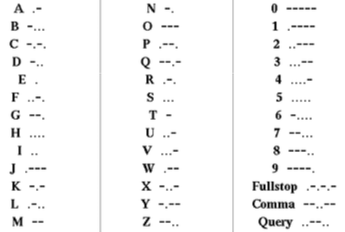
\includegraphics[scale=0.5]{apendice/problemas/problema1a/fig2.png}
\caption{Alfabeto \textit{Morse}}
\label{fig2}
\end{figure}

\subsection{Produto}
Um relatório no modelo de artigos da SBC com uma discussão detalhada sobre as três perguntas levantadas
e sobre a criptografia simplificada.
\subsection{Cronograma}

1 sessão tutorial e 1 aula expositiva.

\subsection{Recursos para aprendizagem}

\noindent
RAMOS, M. V. M.; JOSÉ NETO, J.; VEGA, I. S. \textbf{Linguagens Formais: Teoria, Modelagem e Implementação}. Editora Bookman, 2009.\\

\noindent
MENEZES, Paulo Blauth. \textbf{Linguagens formais e autômatos}. 6. ed. Bookman, 2011.\\

\subsection*{Referências}

Este problema é baseado no texto da Wilhelmiina Hamalainen\footnote{\url{https://www.researchgate.net/profile/Wilhelmiina_Haemaelaeinen}}.

\newpage
\section{A torta e o ladrão de pimenta}
\subsection{Problema}
Os estudantes da disciplina de Introdução as Linguagens Formais e Teoria da Computação da UFBA
souberam na primeira aula da disciplina que será utilizada uma metodologia de ensino baseada
em problemas, então, eles resolveram pesquisar um pouco sobre a metodologia.

Os estudantes se reuniram para conversar sobre as coisas que tinham pesquisado.
Um dos estudantes disse que saber inferir informações implícitas em problemas é muito relevante
para que consigam obter bons resultados.
Outro estudante resolveu contar uma história e os demais ficaram atentos nos mínimos detalhes.

O estudante que conta a história diz que tudo começou na festa de aniversário da Alice.
Não, não a Alice do País das Maravilhas, mas uma amiga dele chamada de Alice:\\

--- Que tal preparar-nos umas tortas saborosas?---perguntou o Rei de Copas à Rainha de Copas num dia fresco de verão.

--- Fazer as tortas sem pimenta?---perguntou a Rainha.

--- Pimenta!---exclamou o Rei, incrédulo---Quer dizer que você usa pimenta em suas tortas?

--- Não muita---respondeu a Rainha.

--- E suponho que ela tem sido roubada!

--- É claro!---disse a Rainha---Encontre a pimenta e, quando descobrir quem a roubou, corte-lhe...

--- Vamos, vamos!---disse o Rei.

--- Bem, a pimenta tinha que ser encontrada, é claro. Agora, como todos vocês sabem, as pessoas que roubam pimenta nunca dizem a verdade.

--- O quê?!---disse Alice (não a Alice do País das Maravilhas, mas a Alice dessa festa)---Nunca ouvi falar disso antes!

--- Não ouviu?---perguntei-lhe, com falsa surpresa.

--- É claro que não! E tem mais, não acredito que ninguém mais tenha ouvido! Algum de vocês ouviu falar disso antes?

Todas as crianças abanaram a cabeça negativamente.

--- Bem,---disse eu---para fins desta história, vamos presumir que as pessoas que roubam pimenta nunca dizem a verdade.

--- Está bem---disse Alice, meio relutante.

--- Então, continuando a história, o suspeito mais óbvio era a cozinheira da Duquesa.

No julgamento, ela fez apenas uma declaração:

--- Eu sei quem roubou a pimenta!

--- Supondo que as pessoas que roubam a pi\-men\-ta sempre mentem, a cozinheira é culpada ou inocente?\\

PORTANTO, QUEM ROUBOU A PIMENTA?\\

Bem, os suspeitos seguintes do Rei foram a Lebre de Março, o Chapeleiro Louco e o Leirão. Os soldados foram mandados às casas deles, mas nenhuma pimenta foi encontrada. Mesmo assim, eles poderiam estar escondendo-a em algum lugar, de modo que foram detidos, com base nos princípios gerais.

No julgamento, a Lebre de Março afirmou que o Chapeleiro era inocente e o Chapeleiro afirmou que o Leirão era inocente. O Leirão resmungou uma declaração qualquer enquanto dormia, mas ela não foi registrada.

Como se constatou, nenhum inocente fizera uma afirmação falsa, e (como estamos lembrados) as pessoas que roubam pimenta nunca fazem afirmações verdadeiras. Além disso, a pimenta foi roubada por apenas uma criatura. Qual dos três é o culpado, se é que foi um deles?\\

ENTÃO, QUEM ROUBOU A PIMENTA?\\

--- Ora, ora, esse é realmente um caso difícil---disse o Rei.

Os suspeitos seguintes, curiosamente, foram o Grifo, a Falsa Tartaruga e a Lagosta.

No julgamento, o Grifo afirmou que a Falsa Tartaruga era inocente, e a Falsa Tartaruga disse que a Lagosta era culpada.
Mais uma vez, nenhum inocente mentiu e nenhum culpado disse a verdade.

Quem roubou a pimenta?

\subsection{Produto}
Um relatório no modelo de artigos da SBC para discutir se a cozinheira da história é culpada ou
inocente, se a Lebre de Março, o Chapeleiro Louco, o Leirão, o Grifo, a Falsa Tartaruga ou Lagosta
roubaram a pimenta.
É necessário detalhar cada inferência utilizada, por exemplo, ao inocentar ou acusar alguém, mostrar
quais as inferências e fatos utilizados para tal conclusão.

\subsection{Cronograma}
1 sessão tutorial.

\subsection{Recursos para aprendizagem}
Não foram indicados recursos adicionais de aprendizagem.

\section*{Referências}
Este problema é baseado no texto do Raymond Smullyan extraído do livro ``Alice no País dos Enigmas''.

